\section{应用目标与证据基础}
拟议应用是高校 Python 入门课中的受监督反馈。学生需要定位错误并独立完成复测；教师需要控制提示、检查异常和工作量；院系负责采购与接入。这分别涉及使用者、采用者和买方，不能混为一个需求。已有资产是可执行题族、训练基线、程序核验与主题记忆；教师面板、机构权限、LMS 接入、更正删除流程和生产监控尚未开发。

本章参照商业计划指南\cite{businesscambridge}，连接场景、竞争、运营、财务和验证。资料核对截至2026年11月7日，优先使用原始研究、官方统计和产品文档。产品目录仅用于了解形态，不作为收入证据。三类证据分开使用：数据、训练和智能体研究 测量原型行为，外部研究和官网描述其他系统，定价、需求、工时、转化和回款属于商业假设。本项目未进行客户访谈、竞品账号内同题测试、付费教学 API 试验、学校采购或真实学生试点。

拟议流程为导入教师批准的题目、测试和提示范围，先收学生预测或代码，核验事实后分层反馈，异常进入教师复核，将确认的作答写入可更正记录，再给相关复测。初期只支持声明的 Python 子集，不自动评定高风险考试。原 智能体研究 的12场景中7项完整依赖工具模板，并非采用模型教学；后续工程修复和 SFT 部署也未证明已具机构交付能力。

\begin{figure}[htbp]\centering
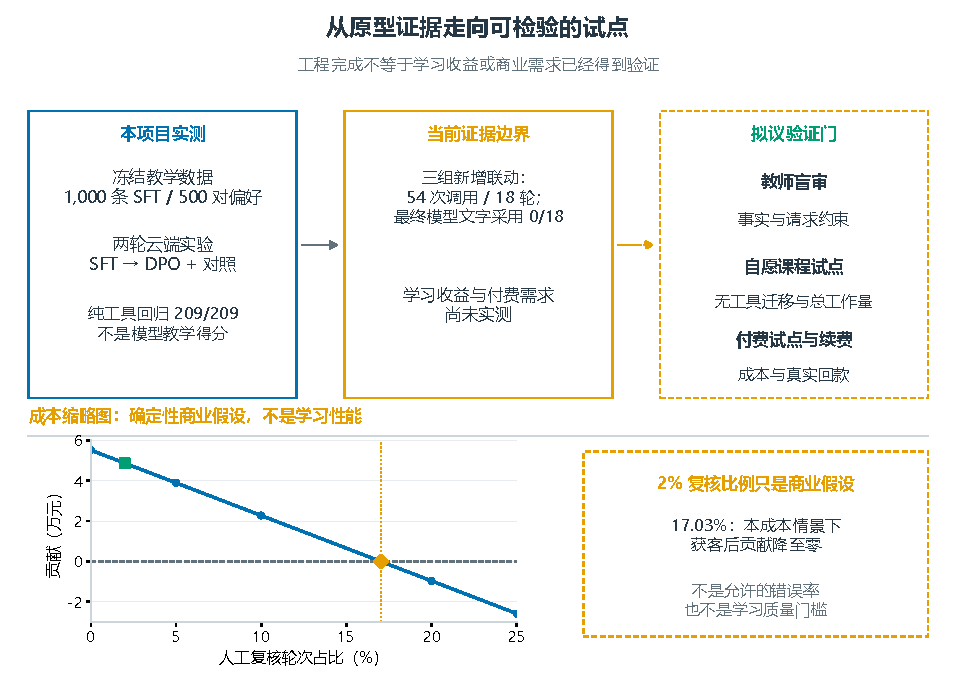
\includegraphics[width=\linewidth]{../../assets/zh/evidence-to-pilot.pdf}
\caption{从研究证据走向拟议受监督试点。实测、供应商公开说明和商业假设的证据作用不同；2\%复核是假设，17.03\%为成本边界，二者都不是实测质量或客户结果。}\label{fig:concise-business-evidence}
\end{figure}\FloatBarrier

\subsection{外部研究能说明什么}
教育部报告2025年高校3167所、高等教育在学规模4872.57万人，包含多种教育形式\cite{businessmoe}。缺少可核验的目标院系、Python 修课人数、预算和采购意愿，不能据此计算已验证市场规模。

Kestin 等的本科物理交叉研究为两周两课，233名选课者中194人纳入，专家设计的 AI 辅导在即时后测上获益\cite{businesskestin}；该系统特定结果不是本项目收益。Bastani 等在土耳其单所高中、近1000名学生的数学试验中发现，无保护 GPT Base 撤去工具后的考试成绩相对对照低约17\%，是相对变化而非百分点；带教学保护的 GPT Tutor 在对应考试结果上也未显示显著正增益\cite{businessbastani}。CodeAid 在700人的编程课程部署12周、分析约8000次交互，强调认知参与和避免直接代写\cite{businesscodeaid}。这些研究支持分别测量有辅助练习、无辅助迁移、延迟保持与教师工时，不能拼成产品排名或付费需求结论。

\section{竞品与差异化假设}
CodeGrade 直接覆盖编程提交、测试、反馈和教师流程；Khanmigo 是范围更广的导师及学校采购比较对象。选择依据是任务相关性，不是市场份额排名。表\ref{tab:concise-business-competitors}依据归档官方说明，未核实某功能不表示该功能不存在。

\begin{table}[htbp]\centering\small
\caption{官方公开能力与当前原型对照（2026年11月7日）。}\label{tab:concise-business-competitors}
\begin{tabularx}{\linewidth}{@{}p{23mm}Y Y Y@{}}\toprule
维度 & CodeGrade & Khanmigo & 本项目\\\midrule
范围 & 编程提交、测试、自动评分 & 跨学科导师、编程辅导、教师和学校方案 & Python 入门研究原型\\
教师与证据控制 & 按作业配置提示和助手；查看会话；代码及学生可见 AutoTest 上下文 & 教师工具和机构接入；本次未核实同类执行轨迹 & 受限解释器、原始审计日志；面板权限未实现\\
接入与记忆 & Advanced/机构方案有 LMS；可看历史，未核实相同主题计数 & 学校名册与单点登录；近期作业摘要，未核实相同计数 & 本地 SQLite；保留 S02 原故障和独立修复；无机构部署\\
采购 & 按课程计划、机构询价 & 免费教师工具、个人订阅、学校询价 & 拟议课程服务；无合同成交证据\\\bottomrule
\end{tabularx}
\par\smallskip\raggedright\scriptsize 来源：CodeGrade 官方价格、产品、帮助、版本说明\cite{businesscgprice,businesscgai,businesscghelp,businesscgrelease}；Khanmigo 价格和 FAQ\cite{businesskhanprice,businesskhan}。公开能力未经过同题账号实测。
\end{table}\FloatBarrier

CodeGrade 免费计划至多50人/课程；Starter 为\$24/学生/课程，Advanced 为\$39，AI 附加项\$15，机构询价\cite{businesscgprice}。读取正文未明确 ISO 币种与税费，保留官网“\$”而不折算人民币。帮助页仍称 Beta，2026年9月版本说明描述付费附加功能，权限须采购时确认\cite{businesscghelp,businesscgrelease}。Khanmigo 教师工具免费，个人/家庭\$4/月或\$44/年、不含销售税，学校询价\cite{businesskhanprice}；个人/家长入口要求成年、美国居住和账单地址，教师工具覆盖更广地区\cite{businesskhan,businesskhangeo}。两家对中国高校的合同、数据驻留和供货条件未核实；个人、课程与机构价格不能直接排序。

通用助手也是替代品。ChatGPT 学习模式公开说明包含免费入口、引导问题、可选记忆及错误和方案限制\cite{businessstudymode}；CodeGrade 已有教师可见和测试上下文。本项目应验证的差异因此是中文课程适配、查错和记录更正的\emph{总负担}是否更低，而非多智能体形式是否新颖。教师授权映射、核验错例和交付经验可能积累，但尚无技术壁垒；现有 LMS 加通用助手应作为实际替代方案比较。

\section{条件化商业模式与单位经济}
假设院系年合同覆盖每学期300人次、两学期共600个“学生--课程”人次，并非600名独立学生。每人次每学期120元，年合同72000元；用量封顶、超额、权限与接入须写入合同。获客拟按教师试点、教研认可、IT审查、预算采购推进；100个待筛院系、20个机会、10次演示、3份合同的漏斗尚无真实名录。年末三份合同对应21.6万元年化合同规模，不是当年到账或已确认收入。

若买方教师时间按90元/小时估值，7.2万元年费需净节省800小时、即每人次80分钟，才能仅靠省时覆盖；20分钟仅值1.8万元/年。这是估值算术，不是实测收益，未减少的固定工资不能当作现金节省。

\subsection{成本模型与压力条件}
假设每人次120轮反馈，\emph{三个角色合计}每轮4500输入、900输出 token，重试系数 $k=1.10$。单价参考百炼 qwen-plus 华北2（北京）、输入至128k、实时非思考公开原价：输入0.8元、输出2元/百万 token，不计优惠\cite{businessprice}。未测试该较大 API 模型的教学或延迟，它也不是第二章训练的0.5B模型。

令 $N$ 为年人次、$s$ 为每人次轮数，$T$ 为合计 token，$p$ 为单价，$r$ 为人工复核比例、$m$ 为分钟、$w$ 为外包时薪，则
\begin{align}
C_{\rm API}&=Nsk\frac{T_{\rm in}p_{\rm in}+T_{\rm out}p_{\rm out}}{10^6},\\
C_{\rm review}&=Nsr\frac{m}{60}w,\\
G&=NP-C_{\rm API}-C_{\rm review}-C_{\rm setup}-C_{\rm cloud}-C_{\rm acquisition}.
\end{align}
合计 token 已含三次调用，不能再乘三。$P$ 为每人次单价，$G$ 扣交付和增量获客、未扣公司固定费用，不是利润或全成本 CAC。基准为2\%复核、每次3分钟、90元/小时、接入80小时、专属云每年1200元、每份新合同获客8000元。变动外包工时不重复计入固定工资；这些数值均不是询价结果。

\begin{figure}[htbp]\centering
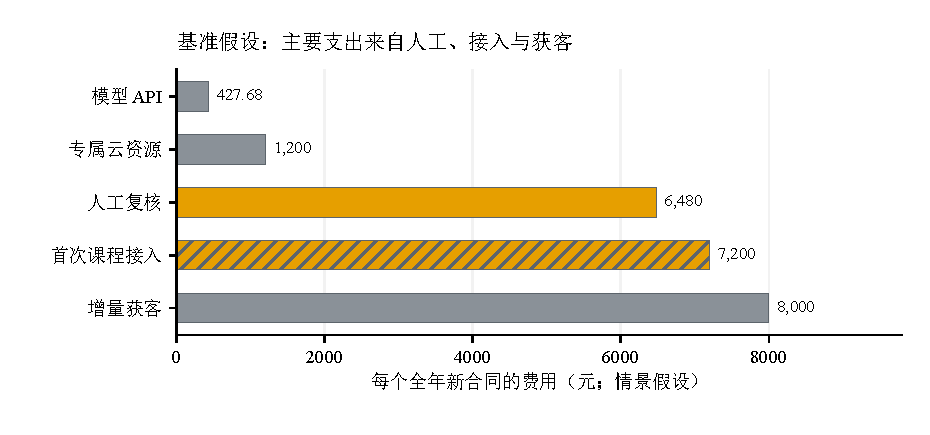
\includegraphics[width=\linewidth]{../../assets/zh/business-costs.pdf}
\caption{基准假设下全年单合同费用。API 为外部单价乘假设用量，人工、接入、云与获客均为规划输入；公司固定费用另计。}\label{fig:concise-business-costs}
\end{figure}\FloatBarrier

\begin{table}[htbp]\centering\small
\caption{基准与联合压力假设。金额为元/全年新合同；完整输入和效率情景保留于补充数据。}\label{tab:concise-business-finance}
\begin{tabularx}{\linewidth}{@{}Yrr@{}}\toprule
项目 & 基准 & 联合压力\\\midrule
每人次单价；每人次轮数 &120；120&90；180\\
复核比例；每次分钟 &2\%；3&5\%；5\\
全年收入 &72000&54000\\
交付成本 &15307.68&54072\\
增量获客 &8000&15000\\
扣交付与获客后贡献 &48692.32&$-15072$\\\bottomrule
\end{tabularx}
\end{table}\FloatBarrier

基准交付包括 API 427.68元、复核6480元、接入7200元、云1200元，扣获客前直接贡献率78.74\%。联合压力还假设接入120小时、云1800元，扩张不能挽救其负贡献。固定支出每年60万元（每月5万，其中人员4.2万），需13份基准全年合同覆盖，连同10万元启动费则需15份；静态全年计算不能当作年中陆续启用的第一年。没有给情景赋概率，也不推算终身价值和续费。

\begin{figure}[htbp]\centering
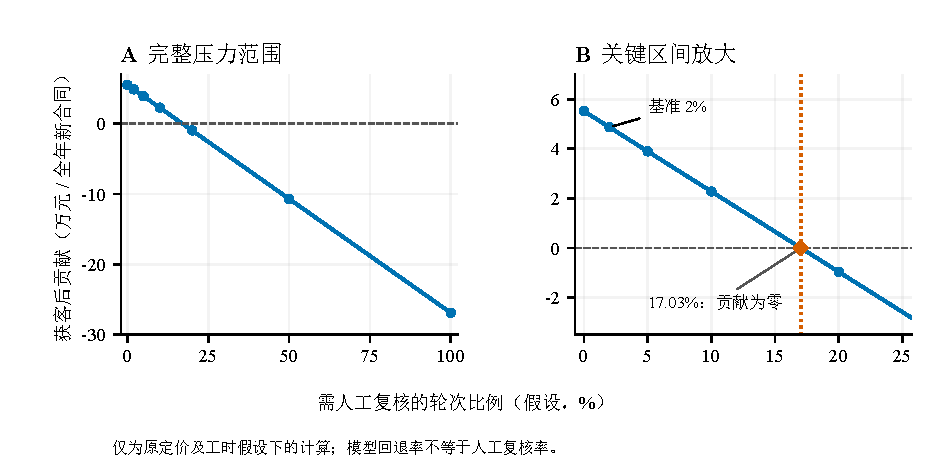
\includegraphics[width=\linewidth]{../../assets/zh/business-review-stress.pdf}
\caption{其余基准不变时的人工复核敏感性。约17.03\%的零贡献点是商业承受边界，不是可接受质量门槛或实测复核率。}\label{fig:concise-business-review}
\end{figure}\FloatBarrier

复核比例10\%、20\%、50\%时，年贡献分别为22772.32、$-9627.68$、$-106827.68$元。模型不采用或回退频次不能直接折算为业务复核概率。若达到质量要求的人工负担超过17.03\%盈亏边界，应调价、缩小范围或停止产品化，不能为了毛利削弱质量保护。

\subsection{现金计划与模拟融资}
模拟融资100万元，支持十二个月工程、试点和采购验证，不设未经依据的估值或退出回报。年合同于第4、7、10月启用，启用时开票，三个月后回款；收入按服务月份摊分，只是规划口径。计划包含首月10万元启动费、每月5万元固定支出，以及启用时的接入获客和使用成本；真实获客费用可能更早发生。

\begin{figure}[htbp]\centering
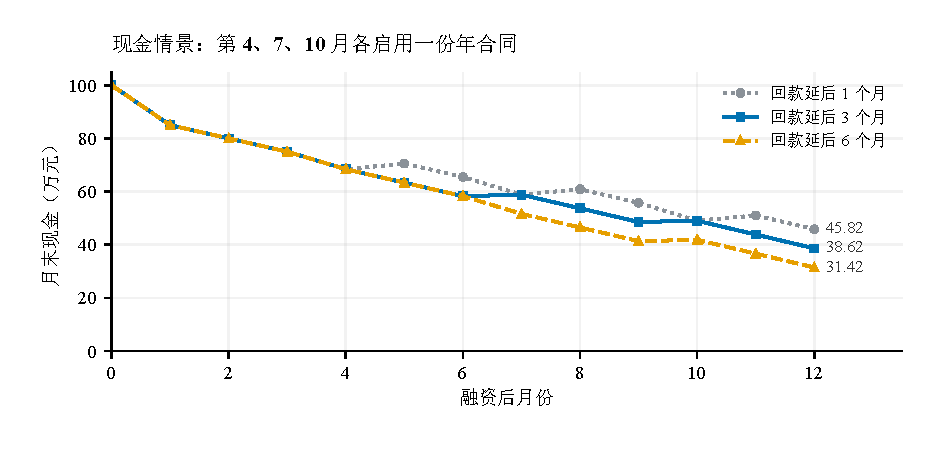
\includegraphics[width=\linewidth]{../../assets/zh/business-cash.pdf}
\caption{融资100万元、分别延迟1、3、6个月回款的现金情景。合同启用与收款均未实际发生。}\label{fig:concise-business-cash}
\end{figure}\FloatBarrier

三个月回款基准首年分摊收入10.8万元、到账14.4万元、年末年化合同21.6万元；支出约75.78万元，余额38.62万元，第10月合同第二年回款。余额须支持后续履约，不是利润。税费、融资、坏账、退款和硬件未计；智能体研究 本机时长不能代表生产延迟或云容量。试点推迟须重算现金流。

\section{验证门槛与决策}
下一步应在补充内容核验后开展受监督试点，而非按日期自动销售。C08/S02 已知输入的工程修复完成；独立教师审阅、学生收益和采购验证尚未开展。

\begin{table}[htbp]\centering\small
\caption{拟议采集与放行条件，均为计划而非已获结果。}\label{tab:concise-business-gates}
\begin{tabularx}{\linewidth}{@{}p{29mm}Y@{}}\toprule
阶段 & 证据与决策边界\\\midrule
内容核验 & 新独立题集和100条教师盲审；严重错误零例才放行，严重误导、越权或记忆污染立即暂停。\\
课程试点 & 两门课约100名自愿学习者，尽量课内随机；计入全部备题、复核、纠错和维护工时，两周后无辅助迁移、盲化阅卷。用于可行性和方差，不保证统计效力。\\
质量与工作量 & 拟议误导率 $\leq2\%$、净节时 $\geq20\%$、后测相对对照不低于 $-5$ 分（满分100）。预登记并报区间，跨门槛视为不确定；独立100条零误导的单侧95\%上界仍为2.95\%；支持2\%误导率门槛至少需149条独立且零误导的审查，同一学生的多条记录未必独立。\\
采购与交付 & 访谈15名教师、5名采购角色；演示前记录现流程，区分拒绝、报价、签约、开票和到账。3个合作意向是目标，不是3个已有客户。\\\bottomrule
\end{tabularx}
\end{table}\FloatBarrier

仅靠20\%净节时抵付假设费用，原工作量须至少达到每人次400分钟；目前尚未测量，否则应调整价格或另证其他收益。严重事件与一般误导率单列。试点需与教师确定门槛，记录交流污染、退出，并用现有课程支持作对照。团队需要工程、课程评价和客户交付职责，不代表已招募人员或建立校方合作。

学生标识和错误历史的未来处理需明确依据、最小字段、期限、更正删除、委托职责和必要影响评估\cite{businesspipl}。伪名、课程权限和更正审计是拟议要求，不是已经完成的合规认证。生产还需代码隔离、并发安全测试、供应商版本和采购数据条款核实。免费替代、适配工时、延期和续费仍有风险；若只能靠密集人工保证质量，应按服务业务如实报价，负贡献则停止扩张。

证据支持有限的受监督验证准备，不支持自主教学、竞品优势或已验证付费意愿。完整网页副本、21项来源台账、三种财务情景、25组敏感性、逐月现金、访谈审查表和计算代码保留在 \path{business/}、\path{business/validation/}。

\paragraph{阅读提示（不属于新实验）。}
“算得出来”只是模型在假设下自洽，不代表有人会买；收入、到账和利润也不是同一件事。特别要看复核人工是否吞掉贡献，以及教师实际省下的时间能否支持价格。图中的17.03\%是成本算出的边界，不能反过来当成教学质量标准。
